\section{Vistas archimate}

A continuación se muestran las vistas generadas por los autores para la muestra de la arquitectura modelada sobre Archimate 2.0. En el capítulo de anexos, en la sección \ref{app:anexo_artefactos}, se puede consultar la descripción de los artefactos que en cada una de ellas aparece.

\subsubsection{Actores y Roles}

\begin{figure}[!htb]
  \begin{center}
    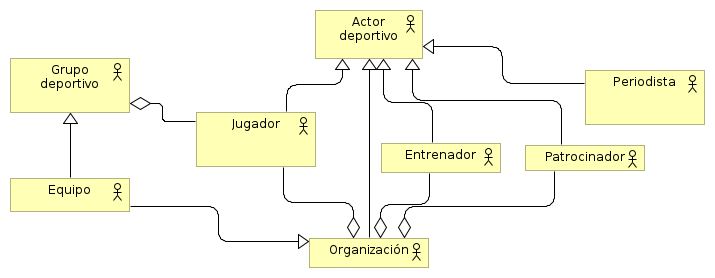
\includegraphics[width=11cm]{./imagenes/actores.png}
    \caption{Actores}
    \label{fig:Actores}
    \textbf{Fuente:}  Autores
  \end{center}
\end{figure}

Aunque esta no es una vista archimate, haciendo uso de esta es posible observar los actores tenidos en cuenta en la creación del SNS. Un actor deportivo es quien desencadena a los demás actores que pueden desenvolverse en la red social debido a las funcionalidades pensadas para ella. El único actor que no ha sido propiamente pensado para ser soportado por la red social, pero que se hace necesario a la hora de tener en claro el negocio, es el periodista. El resto, en su totalidad, son soportados por la red social.

\begin{figure}[!htb]
  \begin{center}
    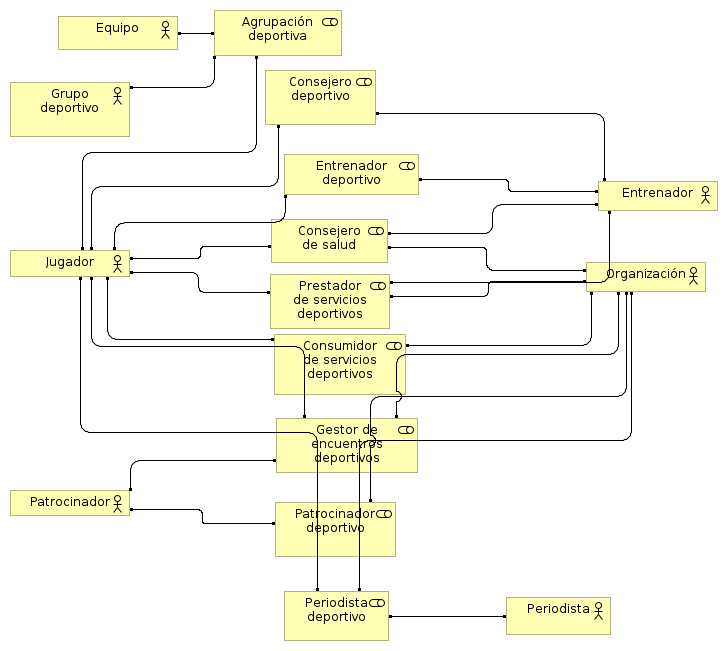
\includegraphics[width=11cm]{./imagenes/roles.png}
    \caption{Roles}
    \label{fig:Roles}
    \textbf{Fuente:}  Autores
  \end{center}
\end{figure}

Es una versión pequeña de un punto de vista organizacional en el que solo se intenta mostrar la relación de asignación entre actores y roles identificados en el diseño de la arquitectura. Debido a la complejidad de una red social deportiva, es posible que un actor adquiera todos los roles mostrados en la vista, sin embargo, especializandose en unos o accediendo principalmente a un rol. Tal es el caso de los roles de agrupación deportiva, entrenador deportivo, prestador de servicios deportivos y patrocinador deportivo.

\subsubsection{Introductory viewpoint}

\begin{figure}[!htb]
  \begin{center}
    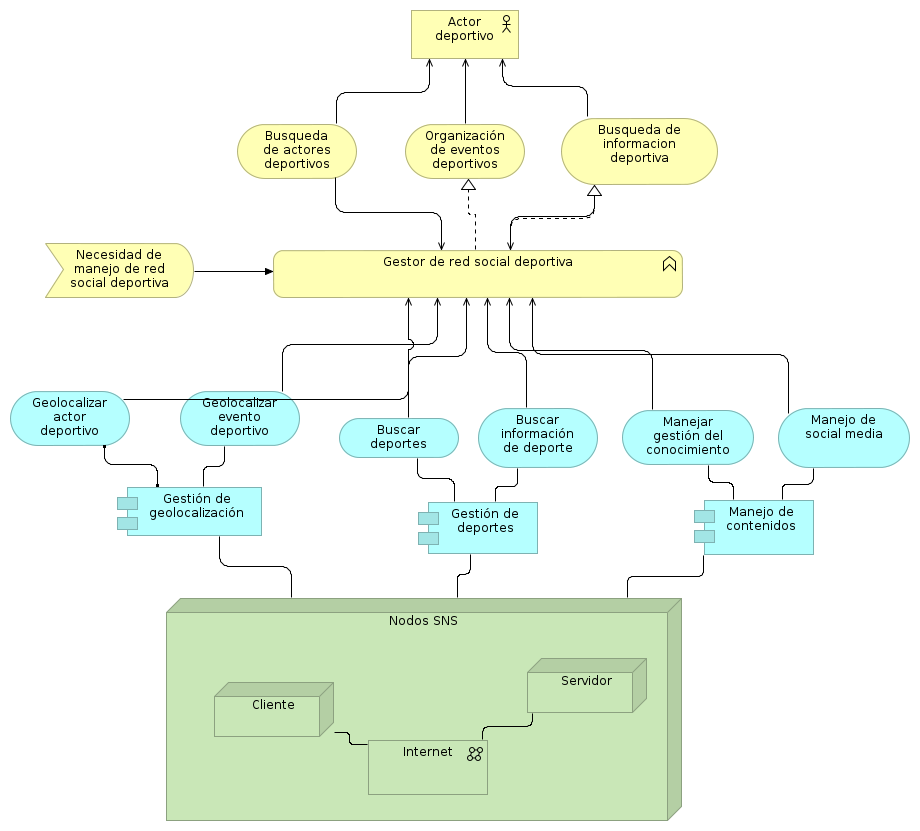
\includegraphics[width=11cm]{./imagenes/introductory.png}
    \caption{Punto de vista introductorio}
    \label{fig:introductory}
    \textbf{Fuente:}  Autores
  \end{center}
\end{figure}

Esta vista muestra las principales características ofrecidas por la red social. Así, es visto que el SNS buscará, en específico, cumplir las funciones de geolocalización, del soporte de información acerca de un deporte, del manejo de social media (esto es, el despliegue de funciones para interactuar con otros en la red social) y el módulo de gestión del conocimiento (similar a la gestión de una comunidad/foro en internet).

\subsubsection{Layered viewpoint}

\begin{figure}[!htb]
  \begin{center}
    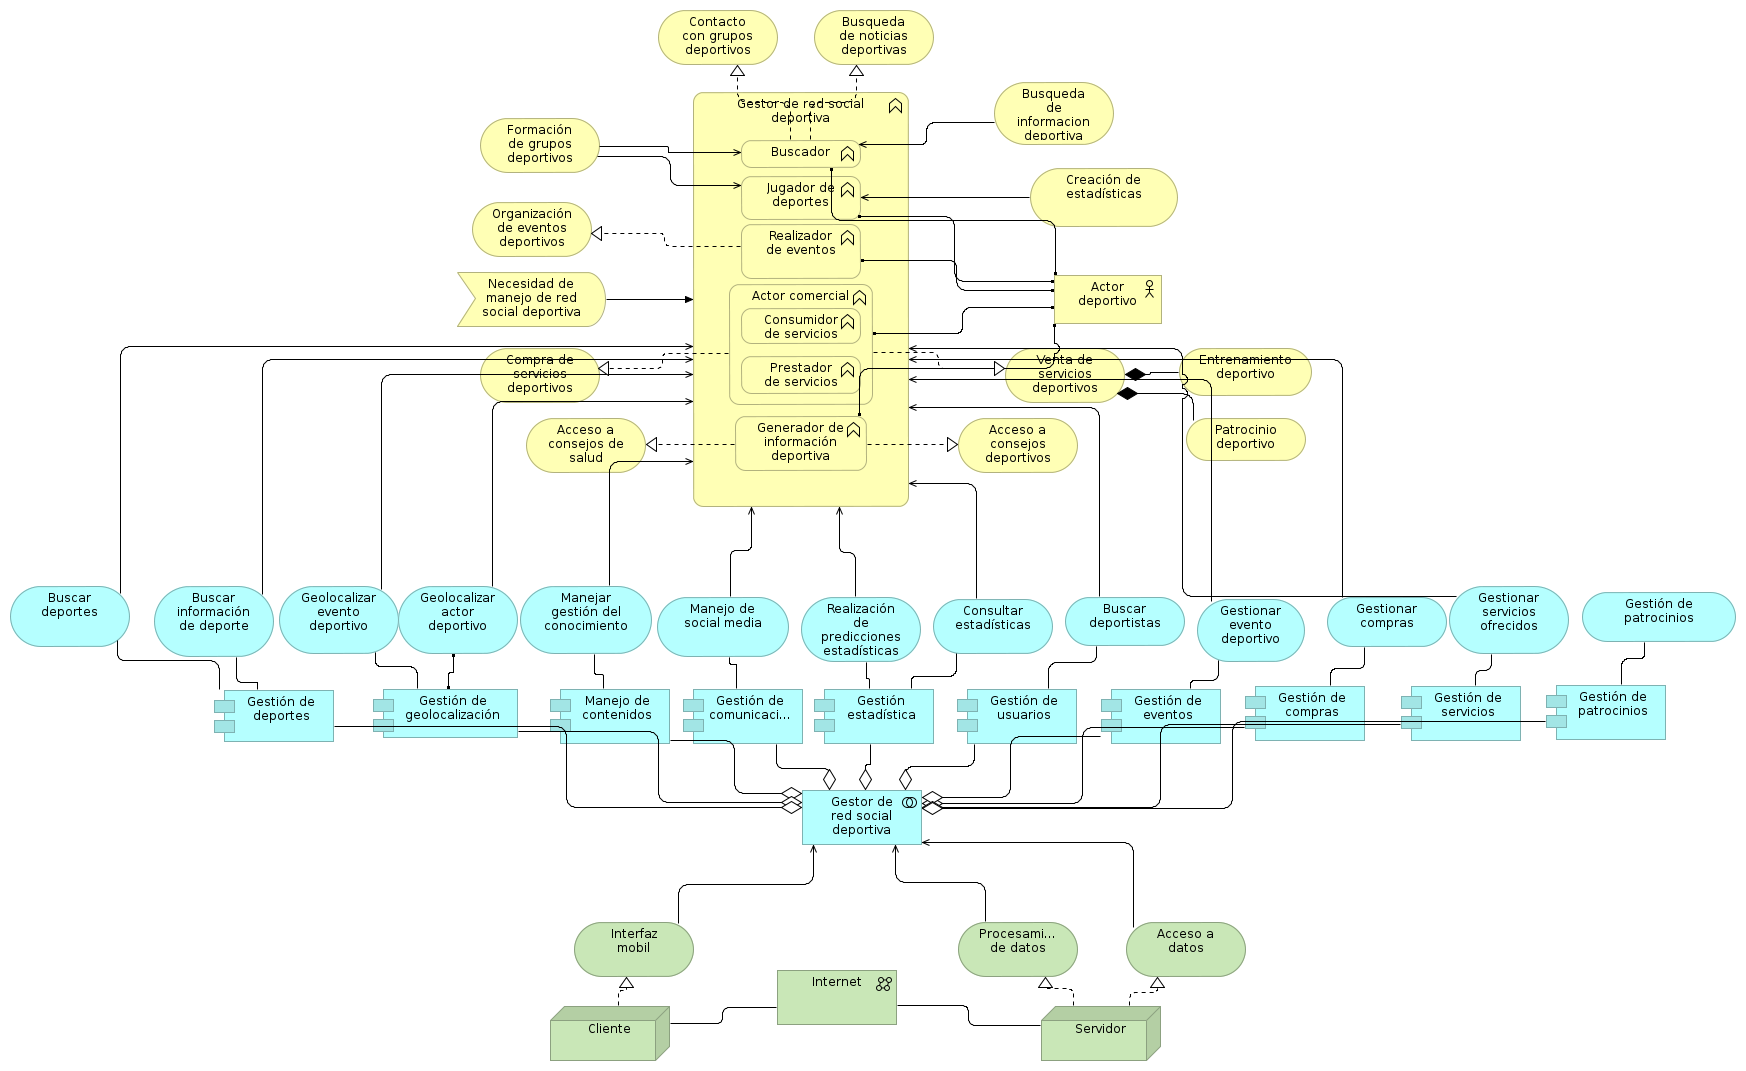
\includegraphics[width=11cm]{./imagenes/generallayered.png}
    \caption{Punto de Vista General por Capas}
    \label{fig:general_layered}
    \textbf{Fuente:}  Autores
  \end{center}
\end{figure}

Este punto de vista es una ampliación del punto de vista introductorio. En este punto de vista es posible observar la visión que han tenido los autores para mostrar una red social deportiva real, todas las funciones que cumple y servicios que realiza/consume un actor deportivo sobre la red. A su vez, es posible observar la ampliación y la aparición de nuevas funcionalidades que soportaría el SNS, teniendo como base la orientación de la red social al deporte amateur o en camino de ser profesional. Entre las nuevas funcionalidades puede observarse la gestión de patrocinios deportivos, la gestión de compra/venta sobre el SNS, la realización de predicciones estadísticas (y, por ende, la producción de las estadísticas mismas) de eventos deportivos y actores deportivos en la red social y la gestión de eventos deportivos. En cuanto al elemento ampliado, se puede observar la ampliación de la geolocalización al ambito de los actores deportivos en la red social así como también de los eventos que en ella se produzcan.

En la capa tecnológica puede observarse la arquitectura cliente/servidor sobre internet, teniendo como terminales los dispositivos móbiles que, en este caso, serán dispositivos Android.

\subsection{Business Functions Viewpoints}

\subsubsection{Organización de Eventos Deportivos}

\begin{figure}[!htb]
  \begin{center}
    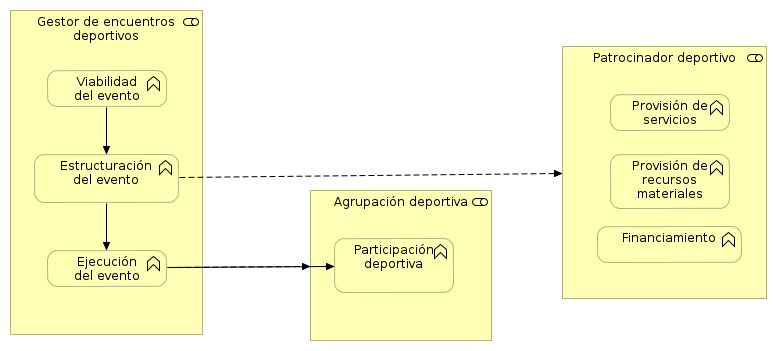
\includegraphics[width=11cm]{./imagenes/business_functions/organizacioneventosdeportivos.png}
    \caption{Organización de Eventos Deportivos}
    \label{fig:bf_organizacion_eventos_deportivos}
    \textbf{Fuente:}  Autores
  \end{center}
\end{figure}

En este punto de vista se puede observar el paso de información a través de los diferentes roles que interactúan en la creación y ejecución de un evento deportivo (patrocinadores, agrupaciones deportivas y gestores de encuentros deportivos) quienes intercambian la información de cada uno para ser patrocinado, para pedir participación o para participar en el evento deportivo.

\subsubsection{Estadísticas Deportivas}

\begin{figure}[!htb]
  \begin{center}
    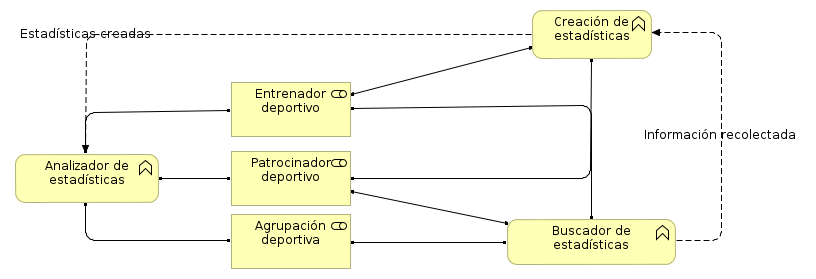
\includegraphics[width=11cm]{./imagenes/business_functions/estadisticasdeportivas.png}
    \caption{Estadísticas Deportivas}
    \label{fig:bf_estadisticas_deportivas}
    \textbf{Fuente:}  Autores
  \end{center}
\end{figure}

Sobre este punto de vista se puede observar que, en específico, entrenadores, patrocinadores deportivos y agrupaciones deportivas producen y utilizan estadísticas. Estas estadísticas son traducidas en calificaciones a los demás en, por ejemplo, el préstamo de servicios deportivos. En el punto de vista de proceso de negocio de estadísticas deportivas es más preciso ver cuales son los tipos de estadística con los cuales se trabaja.

\subsubsection{Buscador Deportivo}

\begin{figure}[!htb]
  \begin{center}
    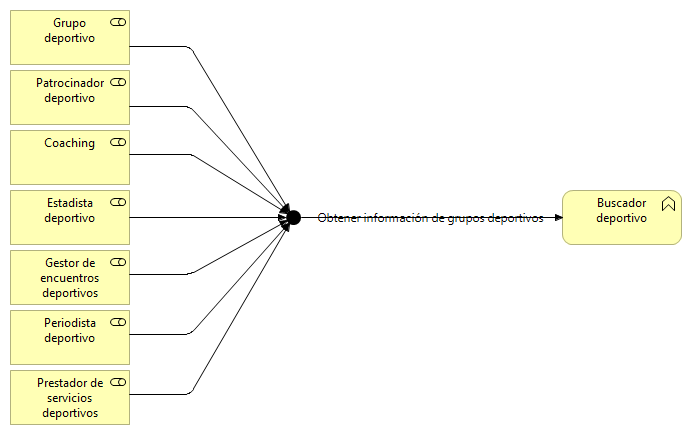
\includegraphics[width=11cm]{./imagenes/business_functions/buscadordeportivo.png}
    \caption{Buscador deportivo}
    \label{fig:BF_BuscadorDeportivo}
    \textbf{Fuente:}  Autores
  \end{center}
\end{figure}

\subsubsection{Consejos}

\begin{figure}[!htb]
  \begin{center}
    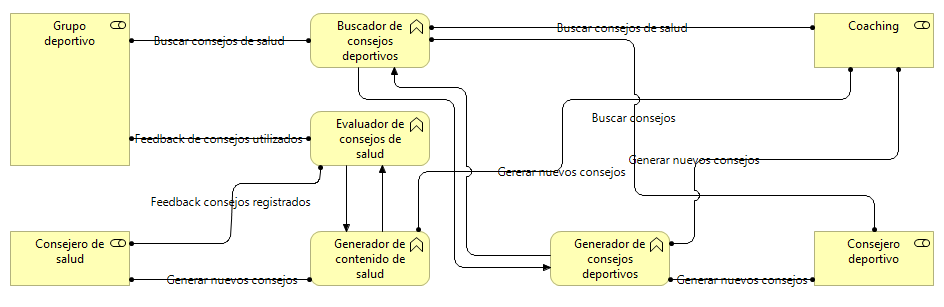
\includegraphics[width=11cm]{./imagenes/business_functions/Consejos.png}
    \caption{Consejos}
    \label{fig:BF_Consejos}
    \textbf{Fuente:}  Autores
  \end{center}
\end{figure}

\subsubsection{Periodismo}

\begin{figure}[!htb]
  \begin{center}
    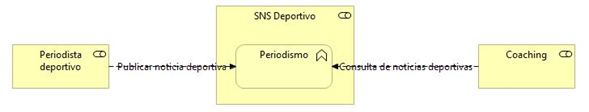
\includegraphics[width=11cm]{./imagenes/business_functions/Periodismo.png}
    \caption{Periodismo}
    \label{fig:BF_Periodismo}
    \textbf{Fuente:}  Autores
  \end{center}
\end{figure}

\subsubsection{Servicios}

\begin{figure}[!htb]
  \begin{center}
    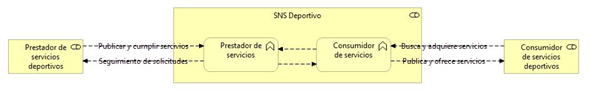
\includegraphics[width=11cm]{./imagenes/business_functions/Servicios.png}
    \caption{Servicios}
    \label{fig:BF_Servicios}
    \textbf{Fuente:}  Autores
  \end{center}
\end{figure}

\subsection{Business Process Viewpoints}

\subsubsection{Organización de Eventos Deportivos}

\begin{figure}[!htb]
  \begin{center}
    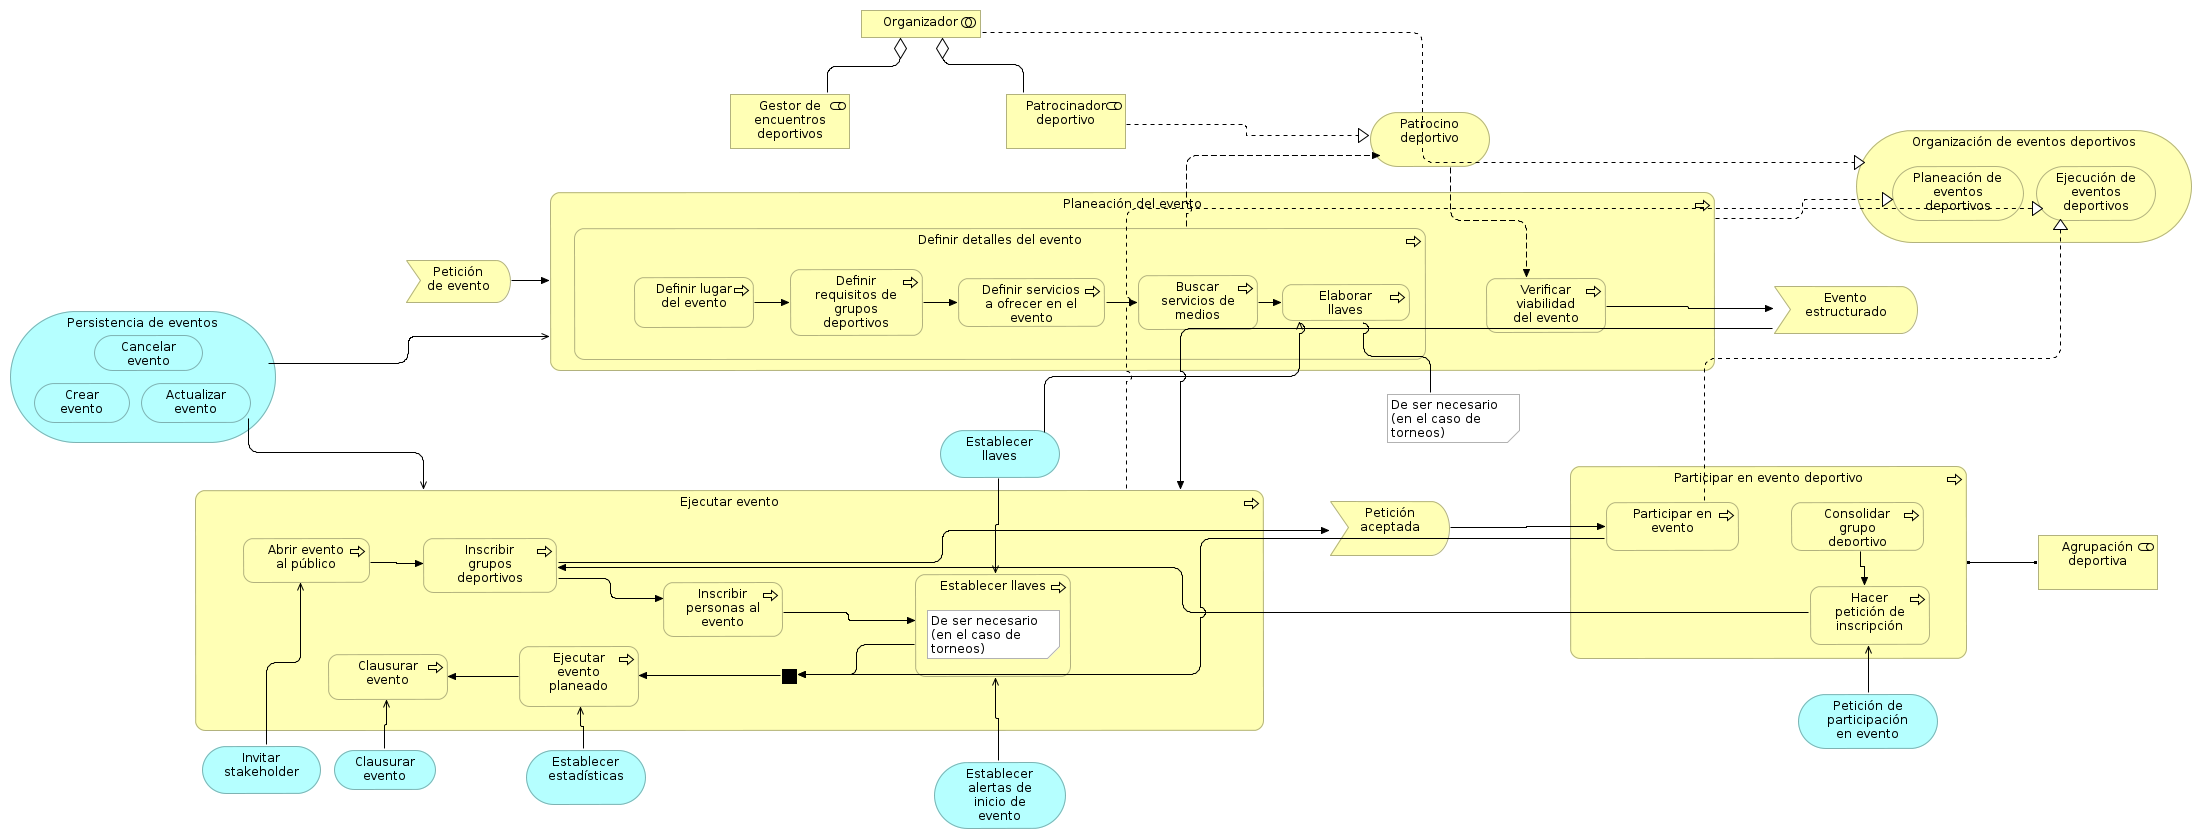
\includegraphics[width=11cm]{./imagenes/business_process/organizacioneventosdeportivos.png}
    \caption{Organización de Eventos Deportivos}
    \label{fig:bp_organizacion_eventos_deportivos}
    \textbf{Fuente:}  Autores
  \end{center}
\end{figure}

En cuanto al proceso de organización de eventos deportivos, los autores han decidido dividir éste en tres procesos grandes: Planear el proyecto, ejecutar el proyecto y participación en el evento deportivo. Se puede ver también que un gestor de eventos deportivos puede trabajar a la par con un patrocinador deportivo para organizar el evento deportivo, con lo cual se puede discernir la conexión entre un patrocinio al evento deportivo y la organización del mismo. El primer gran proceso es soportado por servicios que proporcionan capacidades para tratar con los datos del evento; del segundo gran proceso se soportan algunos de los subprocesos pertenecientes a este, los que son considerados valiosos para el desarrollo del SNS como la invitación y notificación a participantes, así como también la clausura de un evento y la gestión de formatos deportivos; en el tercer gran proceso solo se tienen servicios para la petición a participar en el evento o la participación en el evento mismo.

\subsubsection{Estadísticas Deportivas}

\begin{figure}[!htb]
  \begin{center}
    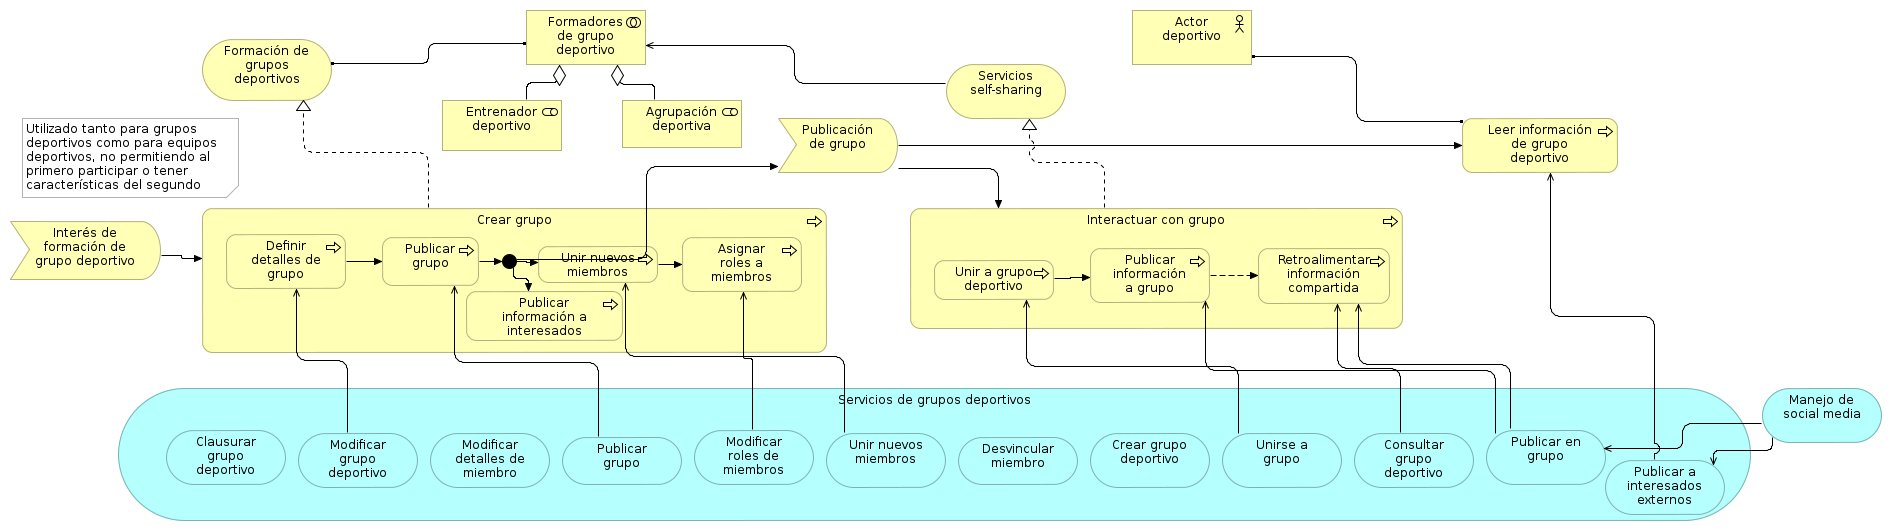
\includegraphics[width=11cm]{./imagenes/business_process/estadisticasdeportivas.png}
    \caption{Estadísticas Deportivas}
    \label{fig:bp_estadisticas_deportivo}
    \textbf{Fuente:}  Autores
  \end{center}
\end{figure}

Esta vista se ha dedicado a expresar el proceso de generación de estadísticas. El diferenciador de este proceso es el tipo de estadísticas que se generan y, por ende, los objetos de negocio que estarán asociados a dichas estadísticas. Las estadísticas generadas serán las de servicios deportivos ofrecidos sobre la red social, sobre estadísticas deportivas de agrupaciones deportivas, sobre estadísticas geoespaciales teniendo en cuenta aspectos de niveles de juego, deportes practicados y eventos generados sobre dicha ubicación geoespacial, y estadísticas propias de un evento deportivo.

En la vista, sobre la capa de aplicación, pueden verse los servicios que soportarán el proceso de generación de estadísticas.

\subsubsection{Buscador de consejos deportivos}

\begin{figure}[!htb]
  \begin{center}
    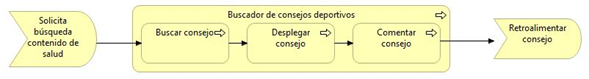
\includegraphics[width=11cm]{./imagenes/business_process/buscadorconsejosdeportivos.png}
    \caption{Buscador de consejos deportivos}
    \label{fig:BP_BuscadorConsejosDeportivos}
    \textbf{Fuente:}  Autores
  \end{center}
\end{figure}

\subsubsection{Buscador deportivo}

\begin{figure}[!htb]
  \begin{center}
    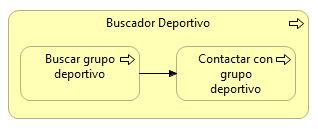
\includegraphics[width=11cm]{./imagenes/business_process/buscadordeportivo.png}
    \caption{Buscador deportivo}
    \label{fig:BP_BuscadorDeportivo}
    \textbf{Fuente:}  Autores
  \end{center}
\end{figure}

\subsubsection{Evaluador consejos de salud}

\begin{figure}[!htb]
  \begin{center}
    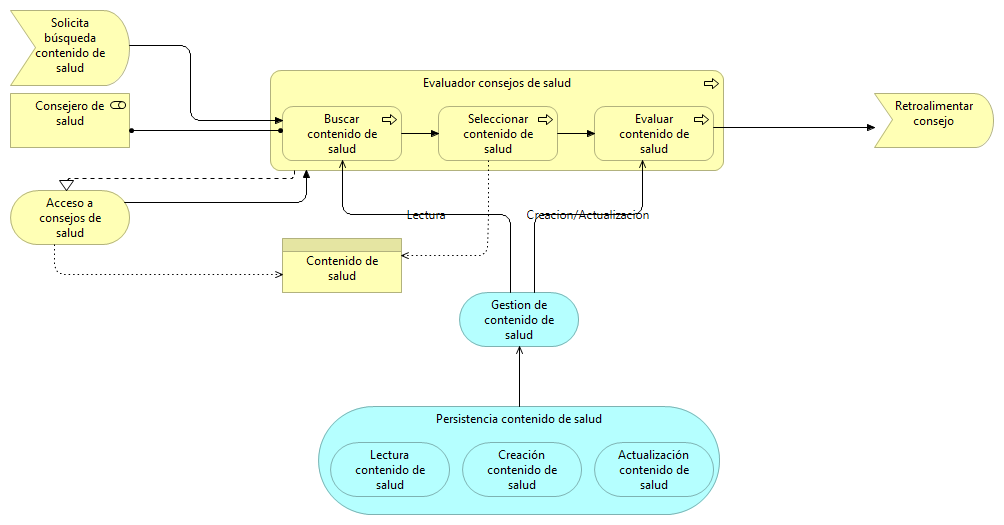
\includegraphics[width=11cm]{./imagenes/business_process/evaluadorconsejossalud.png}
    \caption{Evaluador consejos de salud}
    \label{fig:BP_EvaluadorConsejosSalud}
    \textbf{Fuente:}  Autores
  \end{center}
\end{figure}

\subsubsection{Generador de consejos deportivos}

\begin{figure}[!htb]
  \begin{center}
    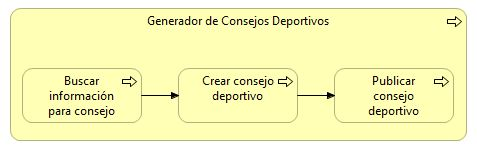
\includegraphics[width=11cm]{./imagenes/business_process/generadorconsejosdeportivos.png}
    \caption{Generador de consejos deportivos}
    \label{fig:BP_GeneradorConsejosDeportivos}
    \textbf{Fuente:}  Autores
  \end{center}
\end{figure}

\subsubsection{Generador de contenidos de salud}

\begin{figure}[!htb]
  \begin{center}
    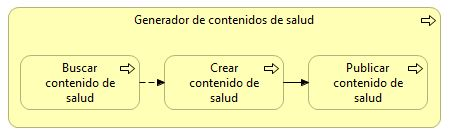
\includegraphics[width=11cm]{./imagenes/business_process/generadorcontenidossalud.png}
    \caption{Generador de contenidos de salud}
    \label{fig:BP_GeneradorContenidosSalud}
    \textbf{Fuente:}  Autores
  \end{center}
\end{figure}

\subsection{Application Usage Viewpoints}

\subsubsection{Organización de Eventos Deportivos}

\begin{figure}[!htb]
  \begin{center}
    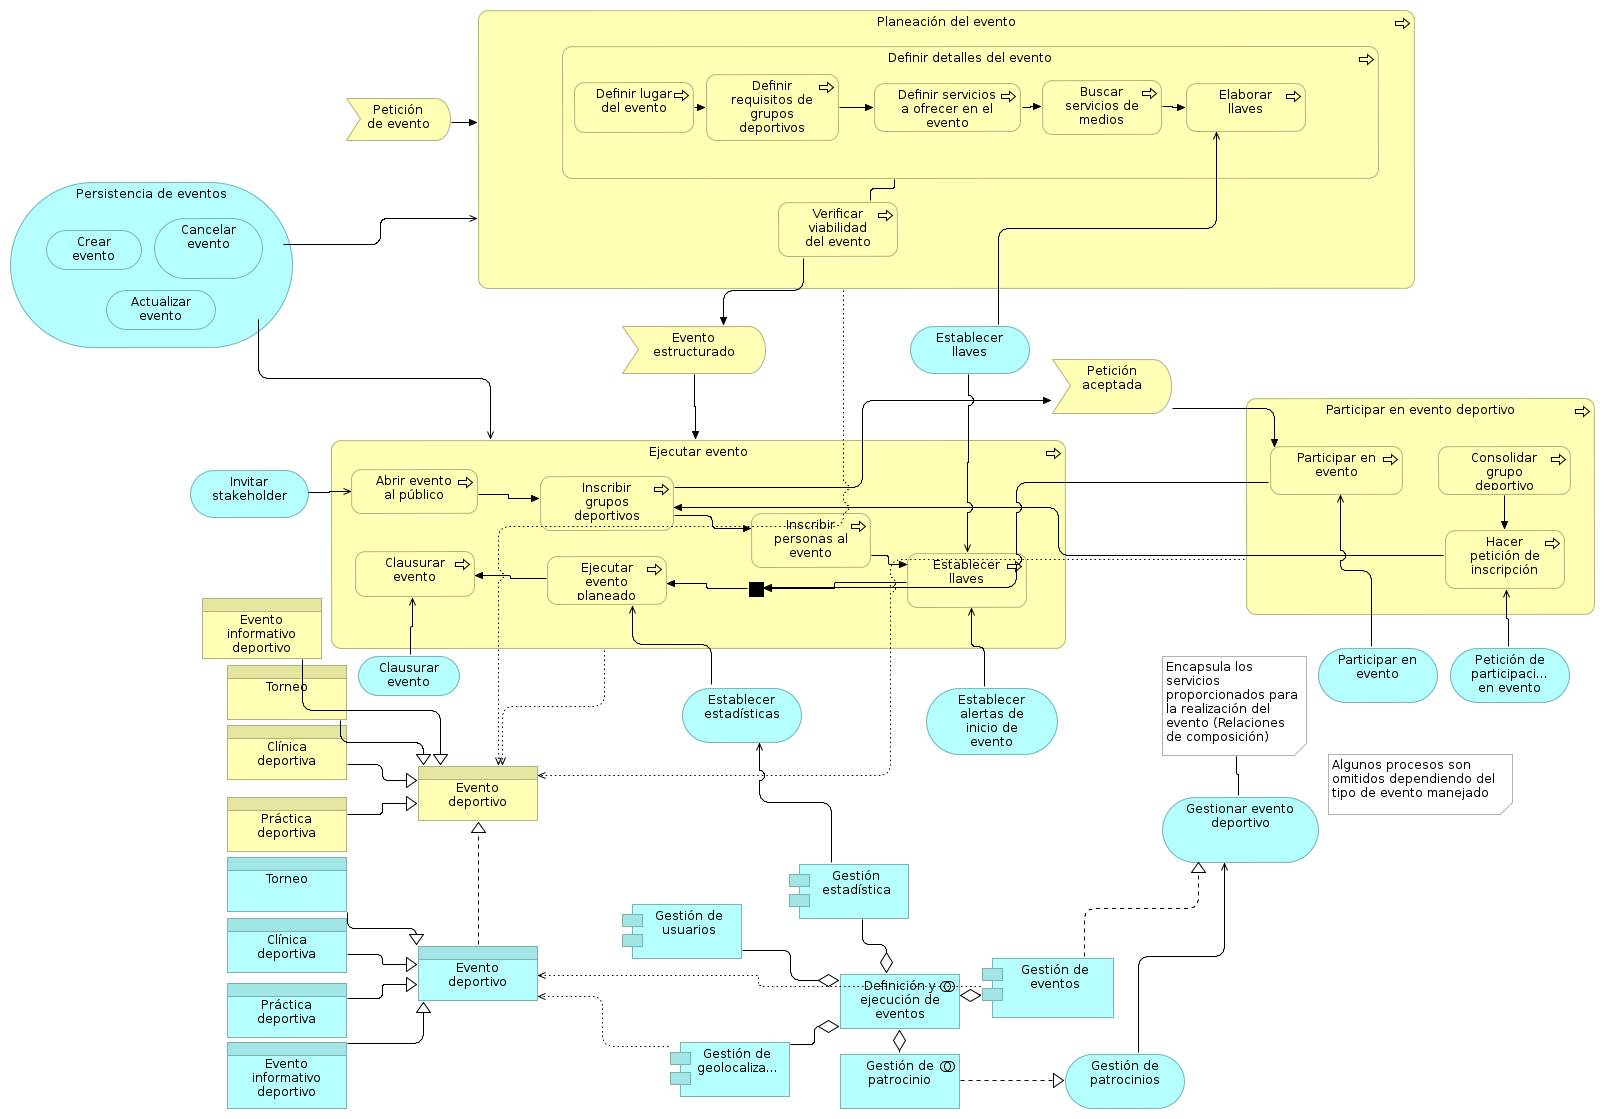
\includegraphics[width=11cm]{./imagenes/application_usage/organizacioneventosdeportivos.png}
    \caption{Organización de Eventos Deportivos}
    \label{fig:au_organizacion_eventos_deportivos}
    \textbf{Fuente:}  Autores
  \end{center}
\end{figure}

Para la organización de eventos deportivos, a parte de lo visto en el punto de vista de proceso de negocio, se puede observar que el SNS deportivo, en una fase final de desarrollo (más allá del prototipo que se alcanza en este proyecto), está dedicado al soporte de funcionalidades para eventos deportivos tales como torneos, clínicas, eventos informativos (como ejemplo, una conferencia deportiva) y, el elemento principal, las prácticas deportivas (prácticas informales realizadas por jugadores amateur).

En soporte de los servicios mostrados, está el componente de gestión de eventos que, junto con la gestión de patrocinio, de geolocalización, de estadísticas y de usuarios.

\subsubsection{Estadísticas Deportivas}

\begin{figure}[!htb]
  \begin{center}
    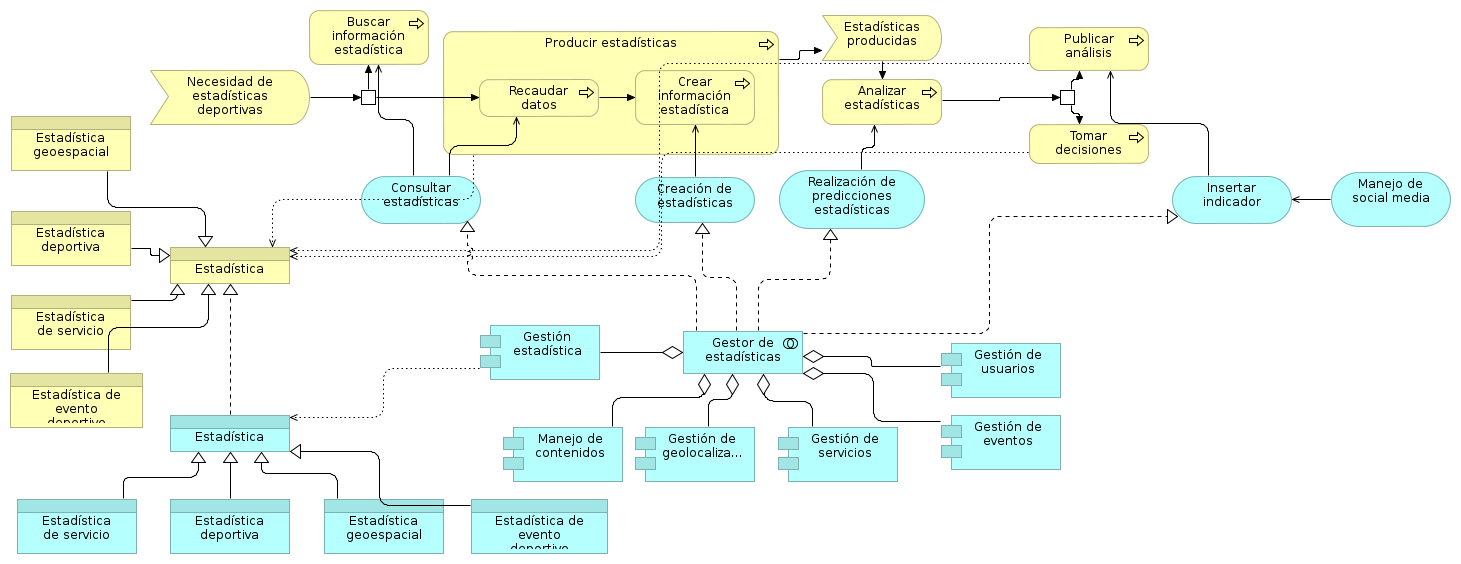
\includegraphics[width=11cm]{./imagenes/application_usage/estadisticasdeportivas.png}
    \caption{Estadísticas Deportivas}
    \label{fig:au_estadisticas_deportivas}
    \textbf{Fuente:}  Autores
  \end{center}
\end{figure}

A parte de lo expresado en el punto de vista de proceso de negocio de estadísticas deportivas, hay múltiples componentes que interactuarán por medio de los servicios que soportan debido al amplio espectro que ocupan las estadísticas sobre el SNS. A parte del componente de gestión de estadísticas, el de usuarios, el de eventos, el de servicios y el de geolocalización ocupan un lugar por ser estos evaluados por medio de estadísticas. Se encuentra también uno de manejo de contenidos que es usado para el compartir las estadísticas y comentar sobre ellas como se haría en la red social deportiva real.

\subsubsection{Buscador de consejos deportivos}

\begin{figure}[!htb]
  \begin{center}
    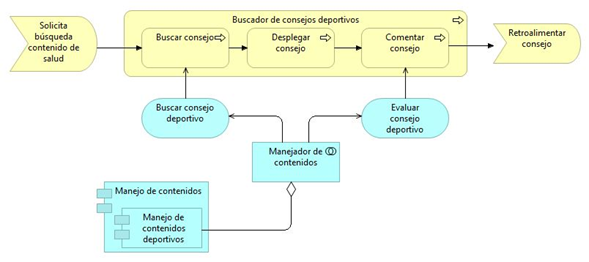
\includegraphics[width=11cm]{./imagenes/application_usage/buscadorconsejosdeportivos.png}
    \caption{Buscador de consejos deportivos}
    \label{fig:BP_BuscadorConsejosDeportivos}
    \textbf{Fuente:}  Autores
  \end{center}
\end{figure}

\subsubsection{Buscador deportivo}

\begin{figure}[!htb]
  \begin{center}
    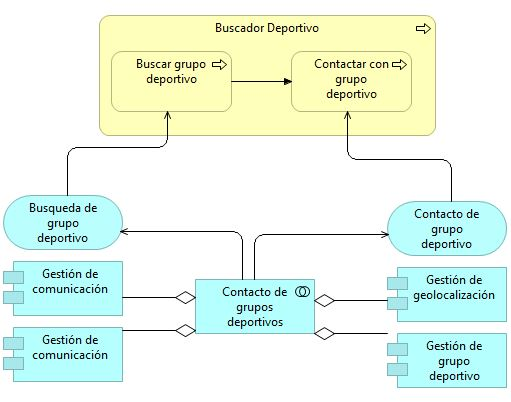
\includegraphics[width=11cm]{./imagenes/application_usage/buscadordeportivo.png}
    \caption{Buscador deportivo}
    \label{fig:BP_BuscadorDeportivo}
    \textbf{Fuente:}  Autores
  \end{center}
\end{figure}

\subsubsection{Evaluador consejos de salud}

\begin{figure}[!htb]
  \begin{center}
    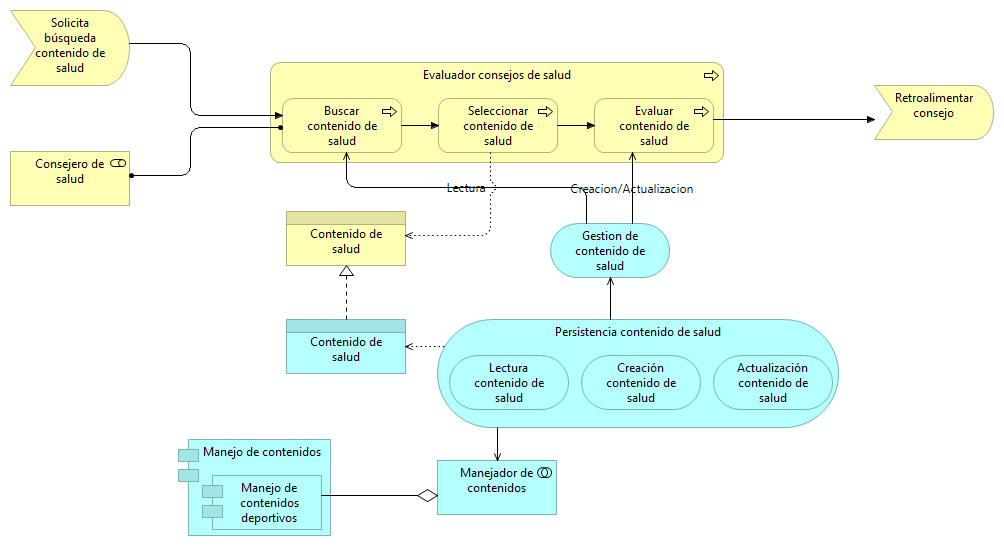
\includegraphics[width=11cm]{./imagenes/application_usage/evaluadorconsejossalud.png}
    \caption{Evaluador consejos de salud}
    \label{fig:BP_EvaluadorConsejosSalud}
    \textbf{Fuente:}  Autores
  \end{center}
\end{figure}

\subsubsection{Generador de consejos deportivos}

\begin{figure}[!htb]
  \begin{center}
    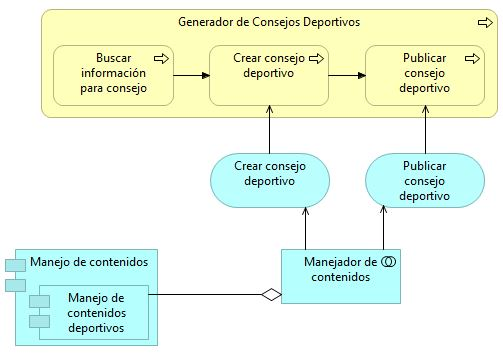
\includegraphics[width=11cm]{./imagenes/application_usage/generadorconsejosdeportivos.png}
    \caption{Generador de consejos deportivos}
    \label{fig:BP_GeneradorConsejosDeportivos}
    \textbf{Fuente:}  Autores
  \end{center}
\end{figure}

\subsubsection{Generador de contenidos de salud}

\begin{figure}[!htb]
  \begin{center}
    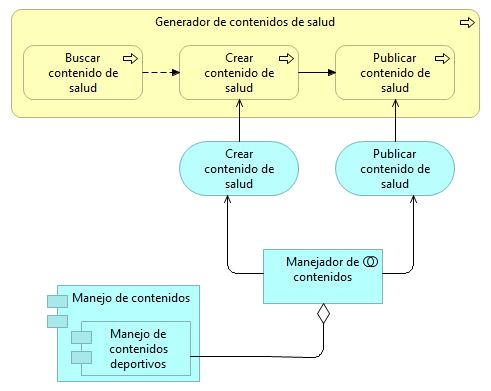
\includegraphics[width=11cm]{./imagenes/application_usage/generadorcontenidossalud.png}
    \caption{Generador de contenidos de salud}
    \label{fig:BP_GeneradorContenidosSalud}
    \textbf{Fuente:}  Autores
  \end{center}
\end{figure}

\subsection{Product Viewpoint}

\subsubsection{Product}

\begin{figure}[!htb]
  \begin{center}
    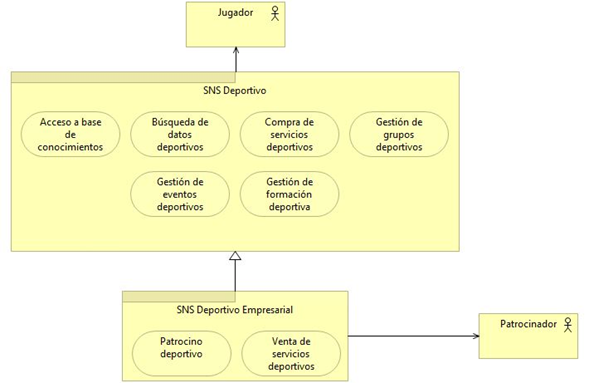
\includegraphics[width=11cm]{./imagenes/Product.png}
    \caption{Producto}
    \label{fig:Product}
    \textbf{Fuente:}  Autores
  \end{center}
\end{figure}

\subsection{Punto de vista de infraestructura}

\begin{figure}[!htb]
  \begin{center}
    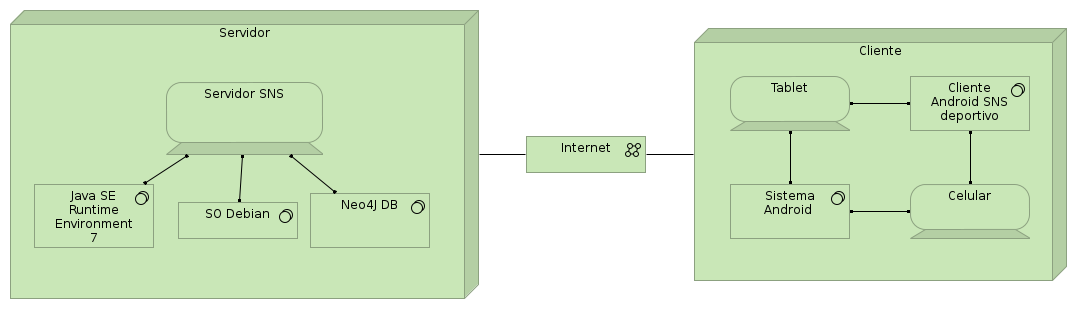
\includegraphics[width=11cm]{./imagenes/infrastructure.png}
    \caption{Punto de vista de infraestructura}
    \label{fig:infrastructure}
    \textbf{Fuente:}  Autores
  \end{center}
\end{figure}

Sobre esta capa se puede observar que los arquitectos han decidido utilizar una arquitectura cliente/servidor para el soporte del desarrollo del SNS. A su vez, se puede observar que el software utilizado por parte del cliente deberá ser un sistema android con el cliente desarrollado específicamente para dar la GUI del SNS. Por parte del servidor se puede ver que se utilizarán entornos Java para el servidor de aplicaciones, Neo4j como la base de datos y sistema operativo Debian. Todo estará soportado sobre conexiones por medio de la red internet.